\documentclass[9pt,twoside,lineno]{pnas-new}
% Use the lineno option to display guide line numbers if required.
\templatetype{pnassupportinginfo}

\usepackage{graphicx}
\usepackage{dcolumn}
\usepackage{bm}
\usepackage{amsfonts}
\usepackage{xcolor,tabu}
\usepackage{multirow}
\usepackage{amsthm}
\usepackage{textcomp}
\usepackage{tikz}
% \usepackage[colorlinks=true,
%             linkcolor=blue,
%             urlcolor=blue,
%             citecolor=blue]{hyperref}
\usepackage{xr}
\usepackage{cleveref}
\usepackage{float}
\usepackage[normalem]{ulem}

% for cross referencing
\makeatletter
\newcommand*{\addFileDependency}[1]{% argument=file name and extension
  \typeout{(#1)}
  \@addtofilelist{#1}
  \IfFileExists{#1}{}{\typeout{No file #1.}}
}
\makeatother

\newcommand*{\myexternaldocument}[1]{%
    \externaldocument{#1}%
    \addFileDependency{#1.tex}%
    \addFileDependency{#1.aux}%
}

\myexternaldocument{correlation}

% add S to figure number
\renewcommand{\thefigure}{S\arabic{figure}}



\title{Density Fluctuations and Energy Spectra of 3D Bacterial Suspensions}
\author{Zhengyang Liu, Wei Zeng, Xiaolei Ma and Xiang Cheng}
\correspondingauthor{Xiang Cheng\\E-mail: xcheng@umn.edu}

\begin{document}

%% Comment out or remove this line before generating final copy for submission; this will also remove the warning re: "Consecutive odd pages found".
% \instructionspage  

% \maketitle

%% Adds the main heading for the SI text. Comment out this line if you do not have any supporting information text.
\SItext

\section{Materials and methods} \label{appendix-MM}
\subsection{Light-powered \textit{E. coli}}
We introduce a light-driven transmembrane proton pump, proteorhodopsin (PR), to wild-type \textit{E. coli} (BW25113) by transforming the bacteria with plasmid pZE-PR encoding the SAR86 $\gamma$-proteobacterial PR-variant \cite{Walter2007}. The activity of PR is correlated with the intensity of light. Thus, we can control the swimming speed of bacteria using light of different intensities. In our experiments, we use high-intensity light, which saturates the light response of bacteria. The average swimming speed of bacteria is fixed at $v_0 = 15 \pm 3$ $\mu$m/s.

The bacteria are cultured at 37 \textcelsius{} with a shaking speed at 250 rpm for 14-16 hours in terrific broth (TB) [tryptone 1.2\% (w/w), yeast extract 2.4\% (w/w), and glycerol 0.4\% (w/w)] supplemented with 0.1 g/L ampicillin. The culture is then diluted 1:100 (v:v) in fresh TB and grown at 30 \textcelsius{} for 6.5 hours. PR expression is triggered by supplementing the culture medium with 1 mM isopropyl $\beta$-D-thiogalactoside and 10  $\mu$M ethanolic all-trans-retinal in the mid-log phase, 3 hours after the dilution.

The bacteria are harvested by gentle centrifugation ($800g$ for 5 min). After discarding the culture medium in the supernatant, we resuspend bacteria with DI water. The resuspended suspension is then centrifuged again at $800g$ for 5 min, and finally adjusted to the target concentration for experiments.

\subsection{Sample preparation and microscopy}

To prepare the sample for microscopy, we construct a seal chamber made of glass slides (25 mm $\times$ 75 mm) and coverslips (18 mm $\times$ 18 mm). We first glue (NOA 81, Norland, NJ) two coverslips on a glass slide, side-by-side, leaving a 3-mm separation between the two coverslips. We then cover the 3-mm separation with another coverslip to form a channel. We pipette bacterial suspensions into the channel. Finally, the two ends of the channel are sealed by UV glue (NOA 76, Norland, NJ) to form a sealed chamber.

Images of the bacterial suspensions are taken 50 $\mu$m above the bottom surface of the sealed chamber by a Nikon Ti-E inverted microscope in the bright-field mode using a 20$\times$ (NA 0.5) objective. The field of view is 420 $\times$ 360 $\mu$m$^2$. All videos are recorded at 30 frames per second using an Andor Zyla sCMOS camera.

\begin{figure}[h]
	\begin{center}
		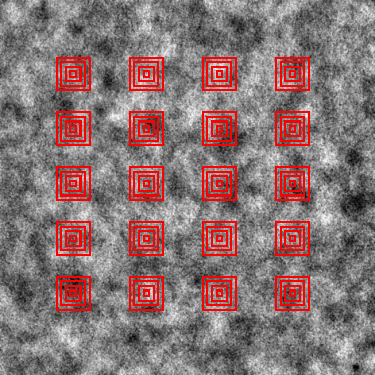
\includegraphics[width=0.4\textwidth]{fig-7.pdf}
		\caption[GNF calculations]
		{Calculation of the standard deviation of the average pixel intensity, $\Delta I$, at different length scales. Density fluctuations are quantified by the standard deviation of the average pixel intensity over time in subsystems of increasing sizes, indicated by the sequences of red squares. Results from twenty different subsystems of the same size evenly distributed in the field of view are then averaged to yield $\Delta I$ for the given subsystem size.}
		\label{GNF-calculation}
	\end{center}
\end{figure}

\FloatBarrier

\section{Image analysis} \label{appendix-IA}
\subsection{Density fluctuations} \label{sec:GNF-calculations}

\subsubsection{Pixel intensity and bacterial number}
In Fig.~\ref{fig:experiment}d, we show that under the same illumination and imaging condition, bacterial density and the average pixel intensity follow approximately a linear relation, which can be expressed as follows:
\begin{equation}
\label{eq:phi-I-relation}
\phi = a + bI,
\end{equation}
where $\phi$ is the volume fraction of bacterial suspensions, $I$ is the average pixel intensity, $a$ and $b$ are constants at the fixed illumination and imaging condition. The number of bacteria in a given subsystem of side length $l$ and thickness $d$ can be calculated as
\begin{equation}
\label{eq:n}
N = \frac{l^2d}{V_b} \phi = \frac{l^2d}{V_b} (a+bI),
\end{equation}
where $V_b$ is the volume of a single bacterium. $d \approx 6$ $\mu$m is the depth of the field of microscopy, which is fixed in our experiments. Thus, the number of bacteria in the subsystem $N$ is proportional to $l^2 \phi$. Taking the standard deviation of both sides of Eq.~\ref{eq:n}, we obtain
\begin{equation}
\label{intensity-number}
\Delta N = \frac{l^2 d}{V_b}|b|\Delta I,
\end{equation}
where $\Delta N$ is the standard deviation of the bacterial number in the subsystem over time and $\Delta I$ is the standard deviation of the average pixel intensity of the subsystem over time. Since $d|b|/V_b$ is a constant independent of subsystem sizes and bacterial volume fractions, $\Delta N$ is linearly proportional to $l^2\Delta I$. Because any constant in front of $\Delta N$ would not affect either the scaling relation or the relative magnitude of density fluctuations at different $\phi$, we simply take $l^2\Delta I$ as $\Delta N$ in our study.

%%%%%%%%

\begin{figure}[t]
	\begin{center}
		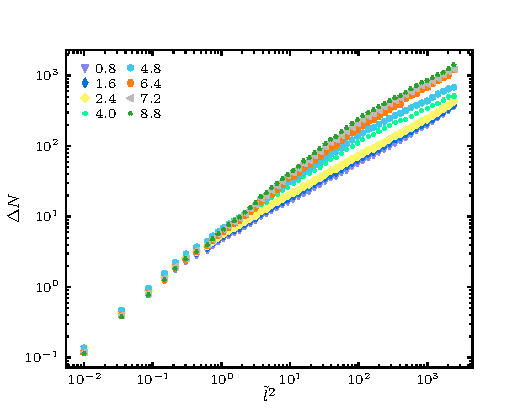
\includegraphics[width=0.47\textwidth]{fig-8.pdf}
		\caption[Density autocorrelation]
		{Calibration of the standard deviation of bacterial number $\Delta N \sim l^2\Delta I$ at different volume fractions $\phi$. $\Delta N$ versus the dimensionless subsystem size $\tilde{l}^2 = l^2/l_b^2$ for bacterial suspensions at different $\phi$. The images are taking under the same illumination with the same imaging condition.
		}
		\label{fig:same-conditions}
	\end{center}
\end{figure}

\FloatBarrier

\subsubsection{Density fluctuations at different length scales}

Based on the linear relation between $\Delta N$ and $\Delta I$, we calculate the density fluctuations at different length scales. We first crop square-shape subsystems of increasing sizes, as shown in Fig.~\ref{GNF-calculation}. For each subsystem size $l$, the standard deviation of the average pixel intensity of the subsystem is calculated over 50 frames (1.67 s or 8.35$\tau_b$), which is longer than the saturated density correlation time of $4\tau_b = 0.8$ s (Fig.~\ref{fig:spatiotemporal-correlations}f). To improve statistics, we choose 20 subsystems of the same size evenly distributed in the field of view and obtain a spatial average of the temporal standard deviation of the average pixel intensity $\Delta I$ (Fig.~\ref{GNF-calculation}). This averaged $\Delta I$ is then multiplied by $l^2$ to give the number density fluctuations $\Delta N$ at the length scale $l$. Note that a second method has also been proposed for calculating number fluctuations, where the standard deviation of particle numbers is computed first spatially over different locations in a single time frame and is then averaged over time of different frames \cite{Aranson2008}.  Although the two methods lead to the same results when spatial and temporal correlations are small compared with the system size and experiment duration \cite{Aranson2008}, the second method is subject to potential systematic errors in our study due to time-independent non-uniform light illumination and intrinsic stationary density variations in non-motile suspensions at $t=0$ in the kinetic measurements. Using the first method, any stable non-uniform light illumination or stationary non-uniform density variations would result in zero temporal standard deviations of $I$ and, therefore, would not affect our measurements of true density fluctuations of motile bacterial suspensions.


\subsubsection{Normalization of bacterial suspensions of different volume fractions}

Practically, to optimize image qualities, we adjust the exposure time of imaging for suspensions of different $\phi$. Exposure times affect the proportional constant $b$ in Eq.~\ref{eq:phi-I-relation}, which introduces a $\phi$-dependent linear constant $b(\phi)$ in Eq.~\ref{eq:n}. Although $b(\phi)$ does not affect the scaling exponent of density fluctuations $\alpha$, it modifies the relative magnitude of $\Delta N$ at different $\phi$. In order to compare the magnitude of density fluctuations at different $\phi$,  we further calibrate and normalize $\Delta I$ for different $\phi$. Specifically, as the calibration, we take videos of bacterial suspensions at different $\phi$ under the exact same imaging condition with fixed illumination light intensity, condenser position, optical filters and all the camera settings such as the exposure time and the dynamic range. The calibration results are shown in Fig.~\ref{fig:same-conditions}, where $\Delta N \sim l^2 \Delta I$ at different $\phi$ collapse at small length scales. The calibration results show that we can normalize $l^2 \Delta I$ of different exposure times by its value at a fixed small length scale. We choose the small scale at $l = 0.3l_b$ in our study. Since $l^2 \Delta I$ at different $\phi$ shows the same slope at small $l$, choosing any other small lengths between $0.1l_b$ and $0.5l_b$ would lead to quantitatively the same results. The normalized density fluctuations show not only the correct scaling exponents but also the right relative magnitudes at different $\phi$.


\subsection{Particle image velocimetry (PIV)} \label{appendix-IA-PIV}

Two-dimensional in-plane velocity fields are extracted by Particle Image Velocimetry (PIV) analysis using the openPIV package in Python \cite{Liberzon2020}. We fix the box size to be 16.5 $\mu$m, which is larger than the size of a single bacterial body but smaller than the velocity correlation length. A step size of the half of the box size with $dx = 8.25$ $\mu$m is used by convention, which sets the spatial resolution of the velocity fields.

\subsection{Energy spectra} \label{appendix-IA-ES}
The energy spectra of bacterial suspensions are calculated as follows. First, we apply the built-in Fast Fourier Transform (FFT) function of Python \texttt{numpy.fft} package to convert the discrete velocity field $\bm{v}(\bm{r}) = [v_x(x,y), v_y(x,y)]$ obtained from PIV to the velocity field in the momentum space $\bm{v_k}(\bm{k}) = [u_k(k_x,k_y),v_k(k_x,k_y)]$. Note that to compensate the difference between FFT and the continuous Fourier transform, we time the $k$-space velocity from FFT by the square of the spatial spacing of the discrete $\bm{v}(\bm{r})$, $dx^2 = 68.1$ $\mu$m$^2$, in order to obtain $\bm{v_k}(\bm{k})$. The point-wise kinetic energy density in the $k$-space is then computed as
\begin{equation}
	E(k_x, k_y) = 
	\frac{1}{2A}\langle u_k(k_x, k_y)u^*_k(k_x, k_y)+v_k(k_x, k_y)v_k^*(k_x, k_y)\rangle
\end{equation}
where $A$ is the total area of the field of view and $^*$ denotes the complex conjugate. $\langle\cdot\rangle$ denotes an average over multiple images from different times. Finally, the energy spectrum $E(k)$ is obtained by summing up $E(k_x,k_y)$ at a constant $k=(k_x^2+k_y^2)^{1/2}$. The approach is mathematically equivalent to the calculation of $E(k)$ from the Fourier transform of the two-point velocity correlation function $\langle \bm{v}(\bm{r_0}) \cdot \bm{v}(\bm{r_0}+\bm{r}) \rangle$. 


\begin{figure}[t]
	\begin{center}
		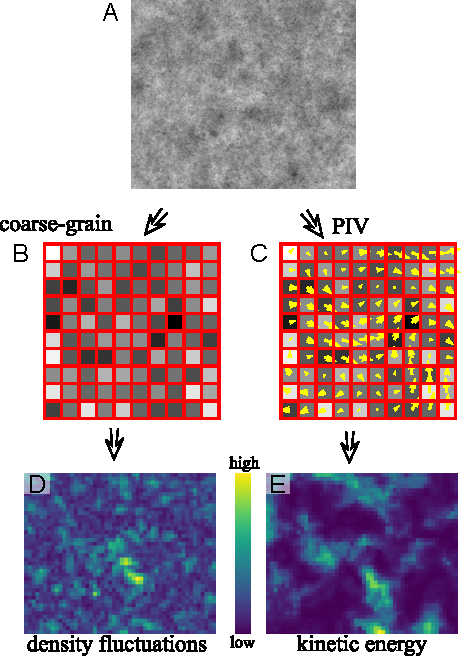
\includegraphics[width=0.46\textwidth]{fig-9.pdf}
		\caption[Density autocorrelation]
		{
			Diagram showing the procedure to calculate the correlation between local density fluctuations and kinetic energies. (a) The raw image of a bacterial suspension at a given time $t$. (b) The coarse-grained image with a pixel size of $l=2.75l_b$. (c) The velocity field from PIV. (d) The field of local density fluctuations, obtained by calculating the standard deviation of the intensity of coarsen-grained pixels shown in (b) over a short time interval. (e) The field of local kinetic energy, obtained by calculating $E = \bm{v}^2/2$ from the velocity field shown in (c).
 		}
		\label{fig:coupling-calculation}
	\end{center}
\end{figure}

\FloatBarrier

\subsection*{Correlation of local density fluctuations and kinetic energies} \label{appendix-IA-localcorrelation}

To calculate local temporal density fluctuations, we need to approximate instantaneous intensity variations. On the one hand, the time interval for calculating the intensity difference between two frames needs to be smaller than the density correlation time ($4\tau_b = 0.8$ s) in order to satisfy the instantaneous approximation. On the other hand, the time interval should be sufficiently long to suppress the influence of random fluctuations of image intensities in adjacent frames. In our study, we choose 0.3 s (10 frames) for the local density fluctuation calculation. We do not expect the results to be much different when varying this number from 0.17 to 0.6 s.

To calculate the local density variations at the length scale of $l = 2.75l_b$ and time $t$, we take 10 consecutive frames following the frame at $t$. All the 10 frames are first coarse-grained by averaging the intensity of pixels in square windows of size $2.75l_b \times 2.75l_b$ into single coarse-grained pixels (Fig.~\ref{fig:coupling-calculation}b). We then take the temporal standard deviation of the coarse-grained pixel intensity over the 10 frames at different positions to obtain a field of density fluctuations at $t$, $\delta N(\bm{r},t)$, as shown in Fig.~\ref{fig:coupling-calculation}d. The same approach has also been used to calculate the field of instantaneous density fluctuations in the transient state shown in Fig.~\ref{fig:GNF-energy-spectra-correlation-transient}a.

Independently, the PIV algorithm is also applied on the original images of the first two frames to obtain the velocity field at time $t$, $\bm{v}(\bm{r},t)$ (Fig.~\ref{fig:coupling-calculation}c). Since the step size of the PIV analysis is also at $2.75l_b$, the velocity field has the same dimensions as the coarse-grained density fluctuation field obtained above. The local kinetic energy can then be calculated as $E(\bm{r},t)=|\bm{v}(\bm{r},t)|^2/2$ (Fig.~\ref{fig:coupling-calculation}e). Finally, the normalized correlation between $\delta N(\bm{r},t)$ and $E(\bm{r},t)$ is computed as
\begin{equation}
C_s = \frac{\langle(\delta N-\overline{\delta N})(E-\overline{E})\rangle}{\sigma_{\delta N}\sigma_{E}},
\end{equation}
where $\bar A$ indicates the mean of variable $A$, $\sigma_A$ indicates the standard deviation of $A$, and $\langle A \rangle$ denotes the average of $A$ over all the positions. The correlation quantifies the spatial similarity between $\delta N$ and $E$, which ranges between $-1$ to 1. Finally, the correlation $C$ shown in Fig.~\ref{fig:GNF-energy-spectra-correlation}b is
calculated by averaging $C_s$ over 1000 frames.


\subsection{Density fluctuations in the transient state} \label{appendix-IA-transient}

Density fluctuations in the transient state towards active turbulence is calculated using the same method as that in the steady state. Specifically, the procedure described in Sec.~\ref{sec:GNF-calculations} is applied at time $t$ over a time interval $\Delta t$ during the transition towards active turbulence. We choose $\Delta t = 1.7$ s (50 frames), which is longer than the density correlation time ($4\tau_b = 0.8$ s) but is significantly smaller than the time of the entire transition ($\sim 60$ s or 1800 frames) for a sufficient temporal resolution.


% \subsection*{Subhead}
% Type or paste text here. This should be additional explanatory text such as an extended technical description of results, full details of mathematical models, etc.   

% \section*{Heading}
% \subsection*{Subhead}
% Type or paste text here. You may break this section up into subheads as needed (e.g., one section on ``Materials'' and one on ``Methods'').

% \subsection*{Materials}
% Add a materials subsection if you need to.

% \subsection*{Methods}
% Add a methods subsection if you need to.


%%% Each figure should be on its own page
% \begin{figure}
% \centering
% \includegraphics[width=\textwidth]{example-image}
% \caption{First figure}
% \end{figure}

% \begin{figure}
% \centering
% \includegraphics[width=\textwidth]{frog}
% \caption{Second figure}
% \end{figure}

% \begin{table}\centering
% \caption{This is a table}

% \begin{tabular}{lrrr}
% Species & CBS & CV & G3 \\
% \midrule
% 1. Acetaldehyde & 0.0 & 0.0 & 0.0 \\
% 2. Vinyl alcohol & 9.1 & 9.6 & 13.5 \\
% 3. Hydroxyethylidene & 50.8 & 51.2 & 54.0\\
% \bottomrule
% \end{tabular}
% \end{table}

%%% Add this line AFTER all your figures and tables
% \FloatBarrier

\movie{The onset of active turbulence in bacterial suspensions (96 s, 4 times of real-time speed, 420x360 $\mu$m$^2$, 6.4\%). Yellow arrows indicates the velocity of the flow field.}

% \movie{Type legend for the other movie here. Adding longer text to show what happens, to decide on alignment and/or indentations.}

% \movie{A third movie, just for kicks.}

% \dataset{dataset_one.txt}{Type or paste legend here.}

% \dataset{dataset_two.txt}{Type or paste legend here. Adding longer text to show what happens, to decide on alignment and/or indentations for multi-line or paragraph captions.}

\bibliography{correlation}

\end{document}



